\subsection{Question 3: Pointing-Error Propagation and the Maximum Travel}\label{sec:q3}

\subsubsection{Model}

Let the vehicle's estimated position be $\hat P=P+\delta$ with independent per-axis
errors $\delta_x,\delta_y\sim N(0,\sigma_{loc}^2(s))$,
$\sigma_{loc}(s)=0.3+0.02s$ (m), where $s$ is the cumulative travel distance since
departure---the standard additive error decomposition of tracking systems
\cite{barshalom2001}. The target is known exactly. Choose local coordinates with true
sightline vector $T-P=(r,0)$ and $r=40$ m. The commanded azimuth is computed from
$\hat P$, giving the exact position-induced angle and total pointing error
\begin{equation}\label{eq:exactgeom}
\alpha=\operatorname{atan2}(-\delta_y,r-\delta_x),\qquad
\Delta\psi=\operatorname{wrap}_{180}(\alpha+\varepsilon_0+\varepsilon_c),
\end{equation}
where the independent gimbal zero bias and control error are
$\varepsilon_0\sim N(0,0.8^{\circ^2})$ and
$\varepsilon_c\sim N(0,0.6^{\circ^2})$.

\emph{Position-induced term.} The position error projects onto the sightline normal as
$\delta_\perp=\delta\cdot n\sim N(0,\sigma_{loc}^2(s))$ (isotropy), and the small-angle
linearization $\alpha\approx\delta_\perp/r$ gives
\begin{equation}\label{eq:loc}
\Delta\psi_{loc}\approx\frac{\delta_\perp}{r}\cdot\frac{180}{\pi}
\;\Rightarrow\;
\sigma_1(s)=\frac{180}{\pi}\cdot\frac{\sigma_{loc}(s)}{40}
=1.4324\,\sigma_{loc}(s)\ \ [\text{deg}] .
\end{equation}
\emph{Synthesis.} Independent Gaussian sources add in variance:
\begin{equation}\label{eq:tot}
\sigma_{tot}(s)=\sqrt{\sigma_1(s)^{2}+0.8^{2}+0.6^{2}},\qquad
P\bigl(|\Delta\psi|\le5^\circ\bigr)=2\Phi\!\Bigl(\frac{5}{\sigma_{tot}(s)}\Bigr)-1 .
\end{equation}
The wrap of $\Delta\psi$ into $[-180^\circ,180^\circ)$ is irrelevant in the feasible
region (verified below).

\emph{Inverse problem.} The reliability requirement
$P\ge0.95$ is equivalent to $z_{0.975}\,\sigma_{tot}\le5$ with $z_{0.975}=1.959964$,
i.e.\ $\sigma_{tot}\le2.551067^\circ$. Peeling Eq.~\eqref{eq:tot} backwards:
$\sigma_1\le2.346901^\circ$, $\sigma_{loc}\le1.638446\,\mathrm{m}$, and with
$\sigma_{loc}(s)=a+bs$ at $s=80$:
\begin{equation}\label{eq:chain}
s_{\max}=\frac{1.638446-0.3}{0.02}=66.9223\ \mathrm{m},
\qquad
a+80\,b\le1.638446,\quad a,b\ge0 .
\end{equation}
The $(a,b)$ feasible set is the right triangle with vertices $(0,0)$, $(1.6384,0)$,
$(0,0.02048)$, shown in Fig.~\ref{fig:q3ab}. The full-geometry check below tightens its
boundary to $a+80b\le1.636745$.

\begin{figure}[!htb]\centering
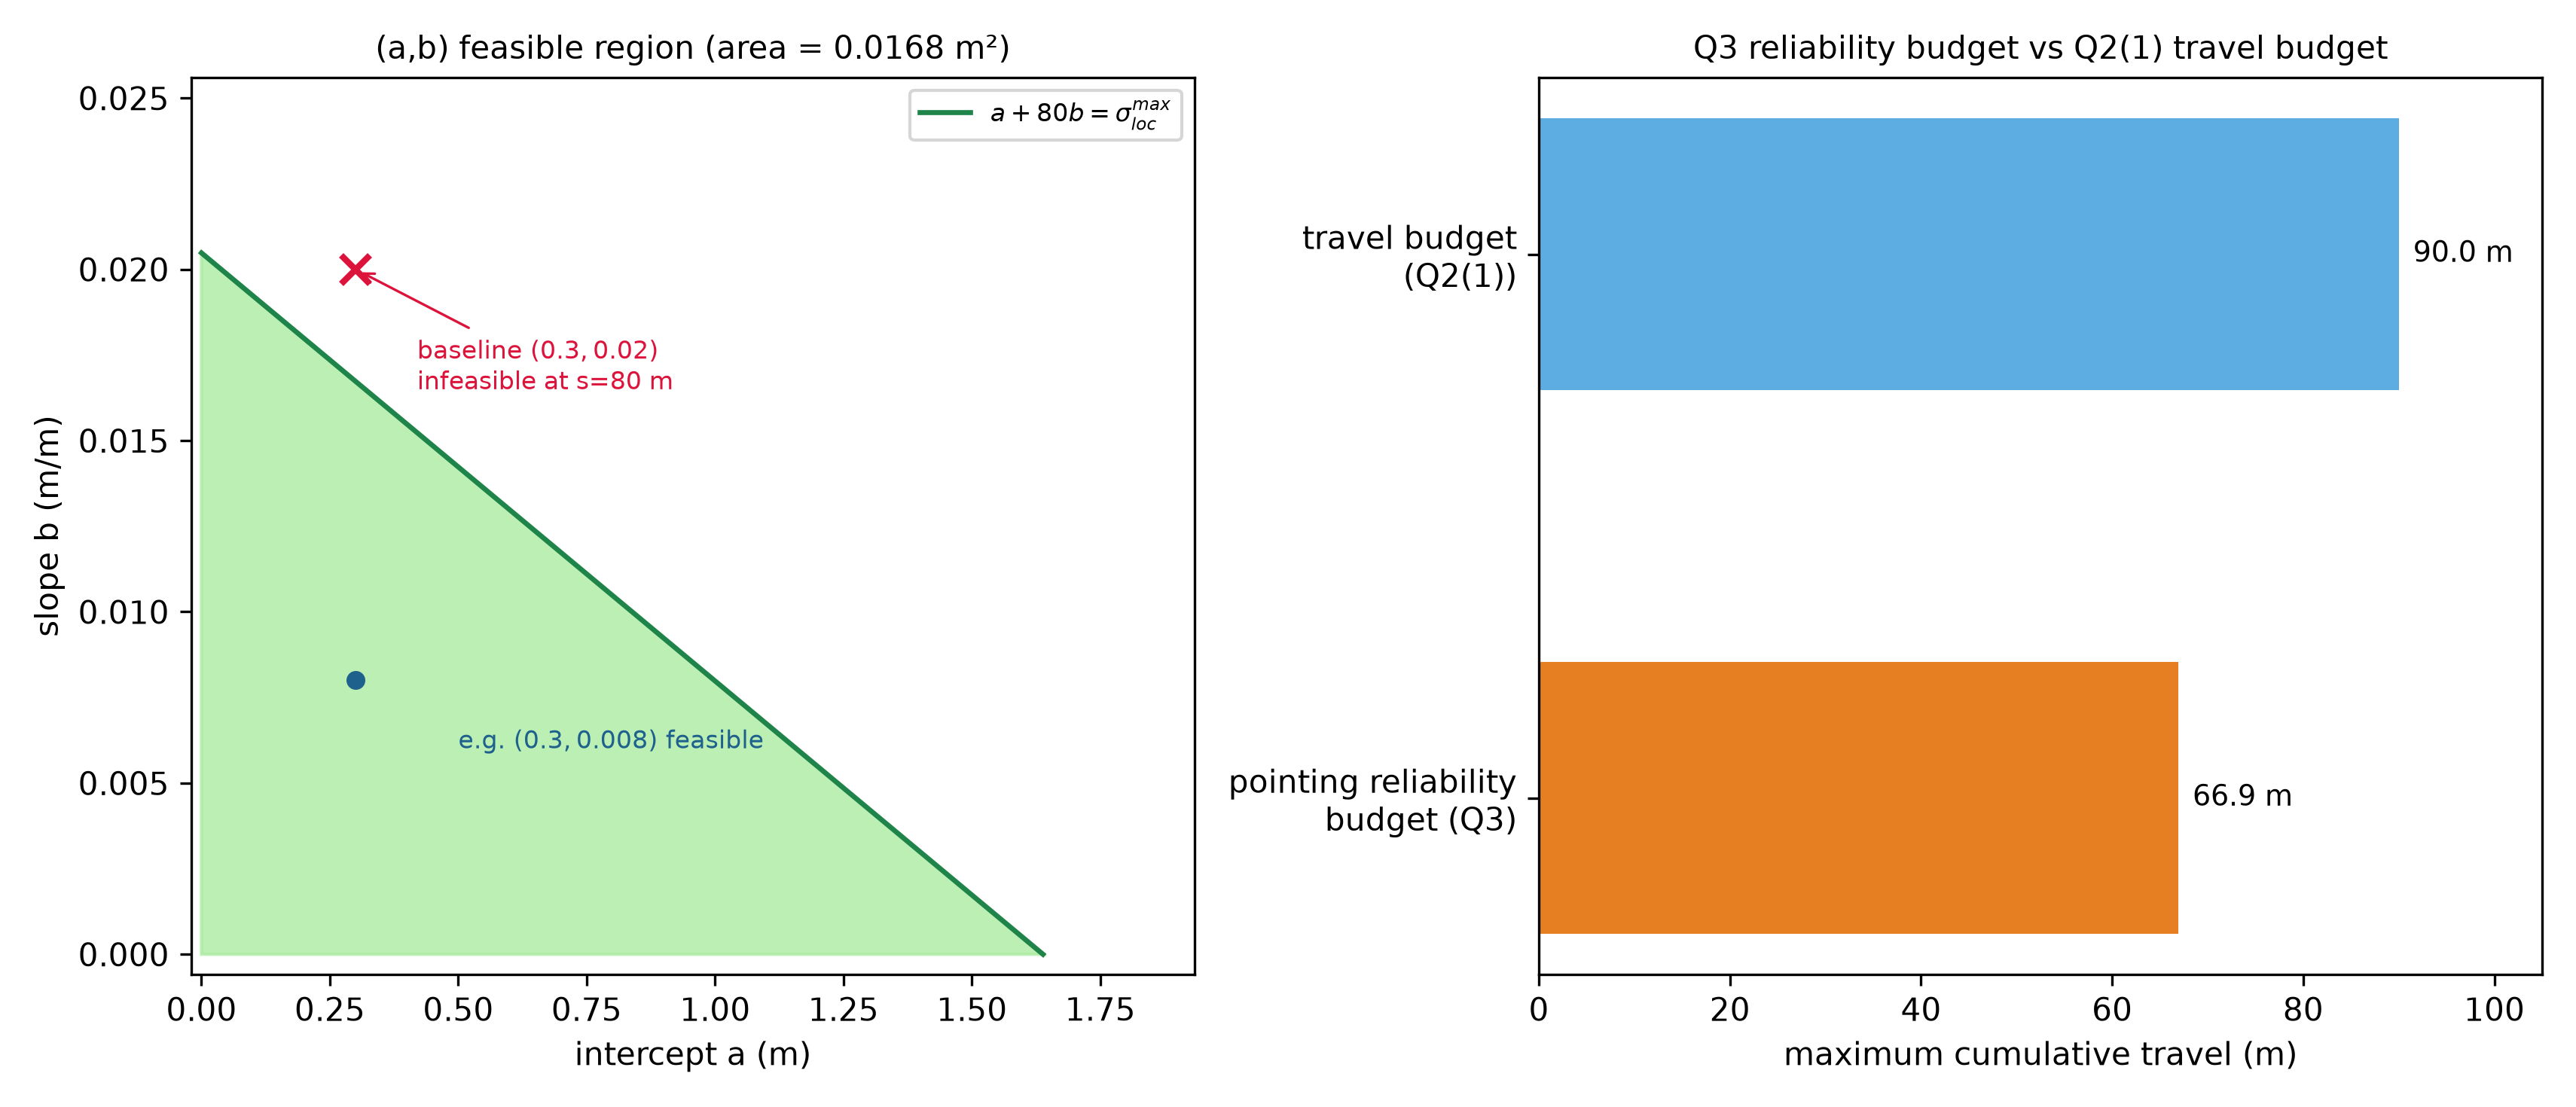
\includegraphics[width=0.39\textwidth]{fig_q3_ab_region.png}
\caption{Feasible region of the error-growth law $(a,b)$ at the 80-m operating point
(shaded): the baseline $(0.3,0.02)$ lies strictly outside---at $80$ m the linearized
pointing reliability would be only $91.54\%$ (full geometry: $91.51\%$).}
\label{fig:q3ab}
\end{figure}

\subsubsection{Justification of the Approximations}

Three approximations enter Eq.~\eqref{eq:loc}--\eqref{eq:tot}.
(i) \emph{Linearization}: arctan nonlinearity and the denominator $r-\delta_x$ have
one-sigma relative scales $0.0559\%$ and $4.0961\%$ at the cap. For $|\alpha|\ge1^\circ$
(avoiding near-zero ratios), the $5\times10^6$-sample diagnostic gives 99th-percentile and
maximum relative errors $10.55\%$ and $20.35\%$; Eq.~\eqref{eq:pexact} below measures
their actual reliability impact.
(ii) \emph{Wrapping}: the linearized tail beyond $180^\circ$ at $80\,\mathrm{m}$ underflows
in double precision, while full \texttt{atan2} and wrap remain in both independent checks.
(iii) \emph{Gaussian synthesis}: exact within the linearized model by independence.

For an approximation-free probability check, let $\lambda(s)=r/\sigma_{loc}(s)$ and
$\sigma_g=\sqrt{0.8^2+0.6^2}=1^\circ$. The exact angle $\alpha$ in
Eq.~\eqref{eq:exactgeom} has density
\begin{equation}\label{eq:angledensity}
f_\lambda(\theta)=\frac{e^{-\lambda^2/2}}{2\pi}
+\frac{\lambda\cos\theta}{\sqrt{2\pi}}\,
e^{-\lambda^2\sin^2\theta/2}\Phi(\lambda\cos\theta),
\qquad -\pi\le\theta\le\pi .
\end{equation}
Convolving this density with the Gaussian gimbal error gives the one-dimensional integral
\begin{equation}\label{eq:pexact}
P_{exact}(s)=\int_{-\pi}^{\pi}f_{\lambda(s)}(\theta)
\left[\Phi\!\left(\frac{5^\circ-\theta_{deg}}{\sigma_g}\right)
-\Phi\!\left(\frac{-5^\circ-\theta_{deg}}{\sigma_g}\right)\right]d\theta,
\quad \theta_{deg}=\frac{180\theta}{\pi},
\end{equation}
which we evaluate by adaptive quadrature, without linearization or sampling error.

\subsubsection{Results and Validation}

\begin{figure}[!htb]\centering
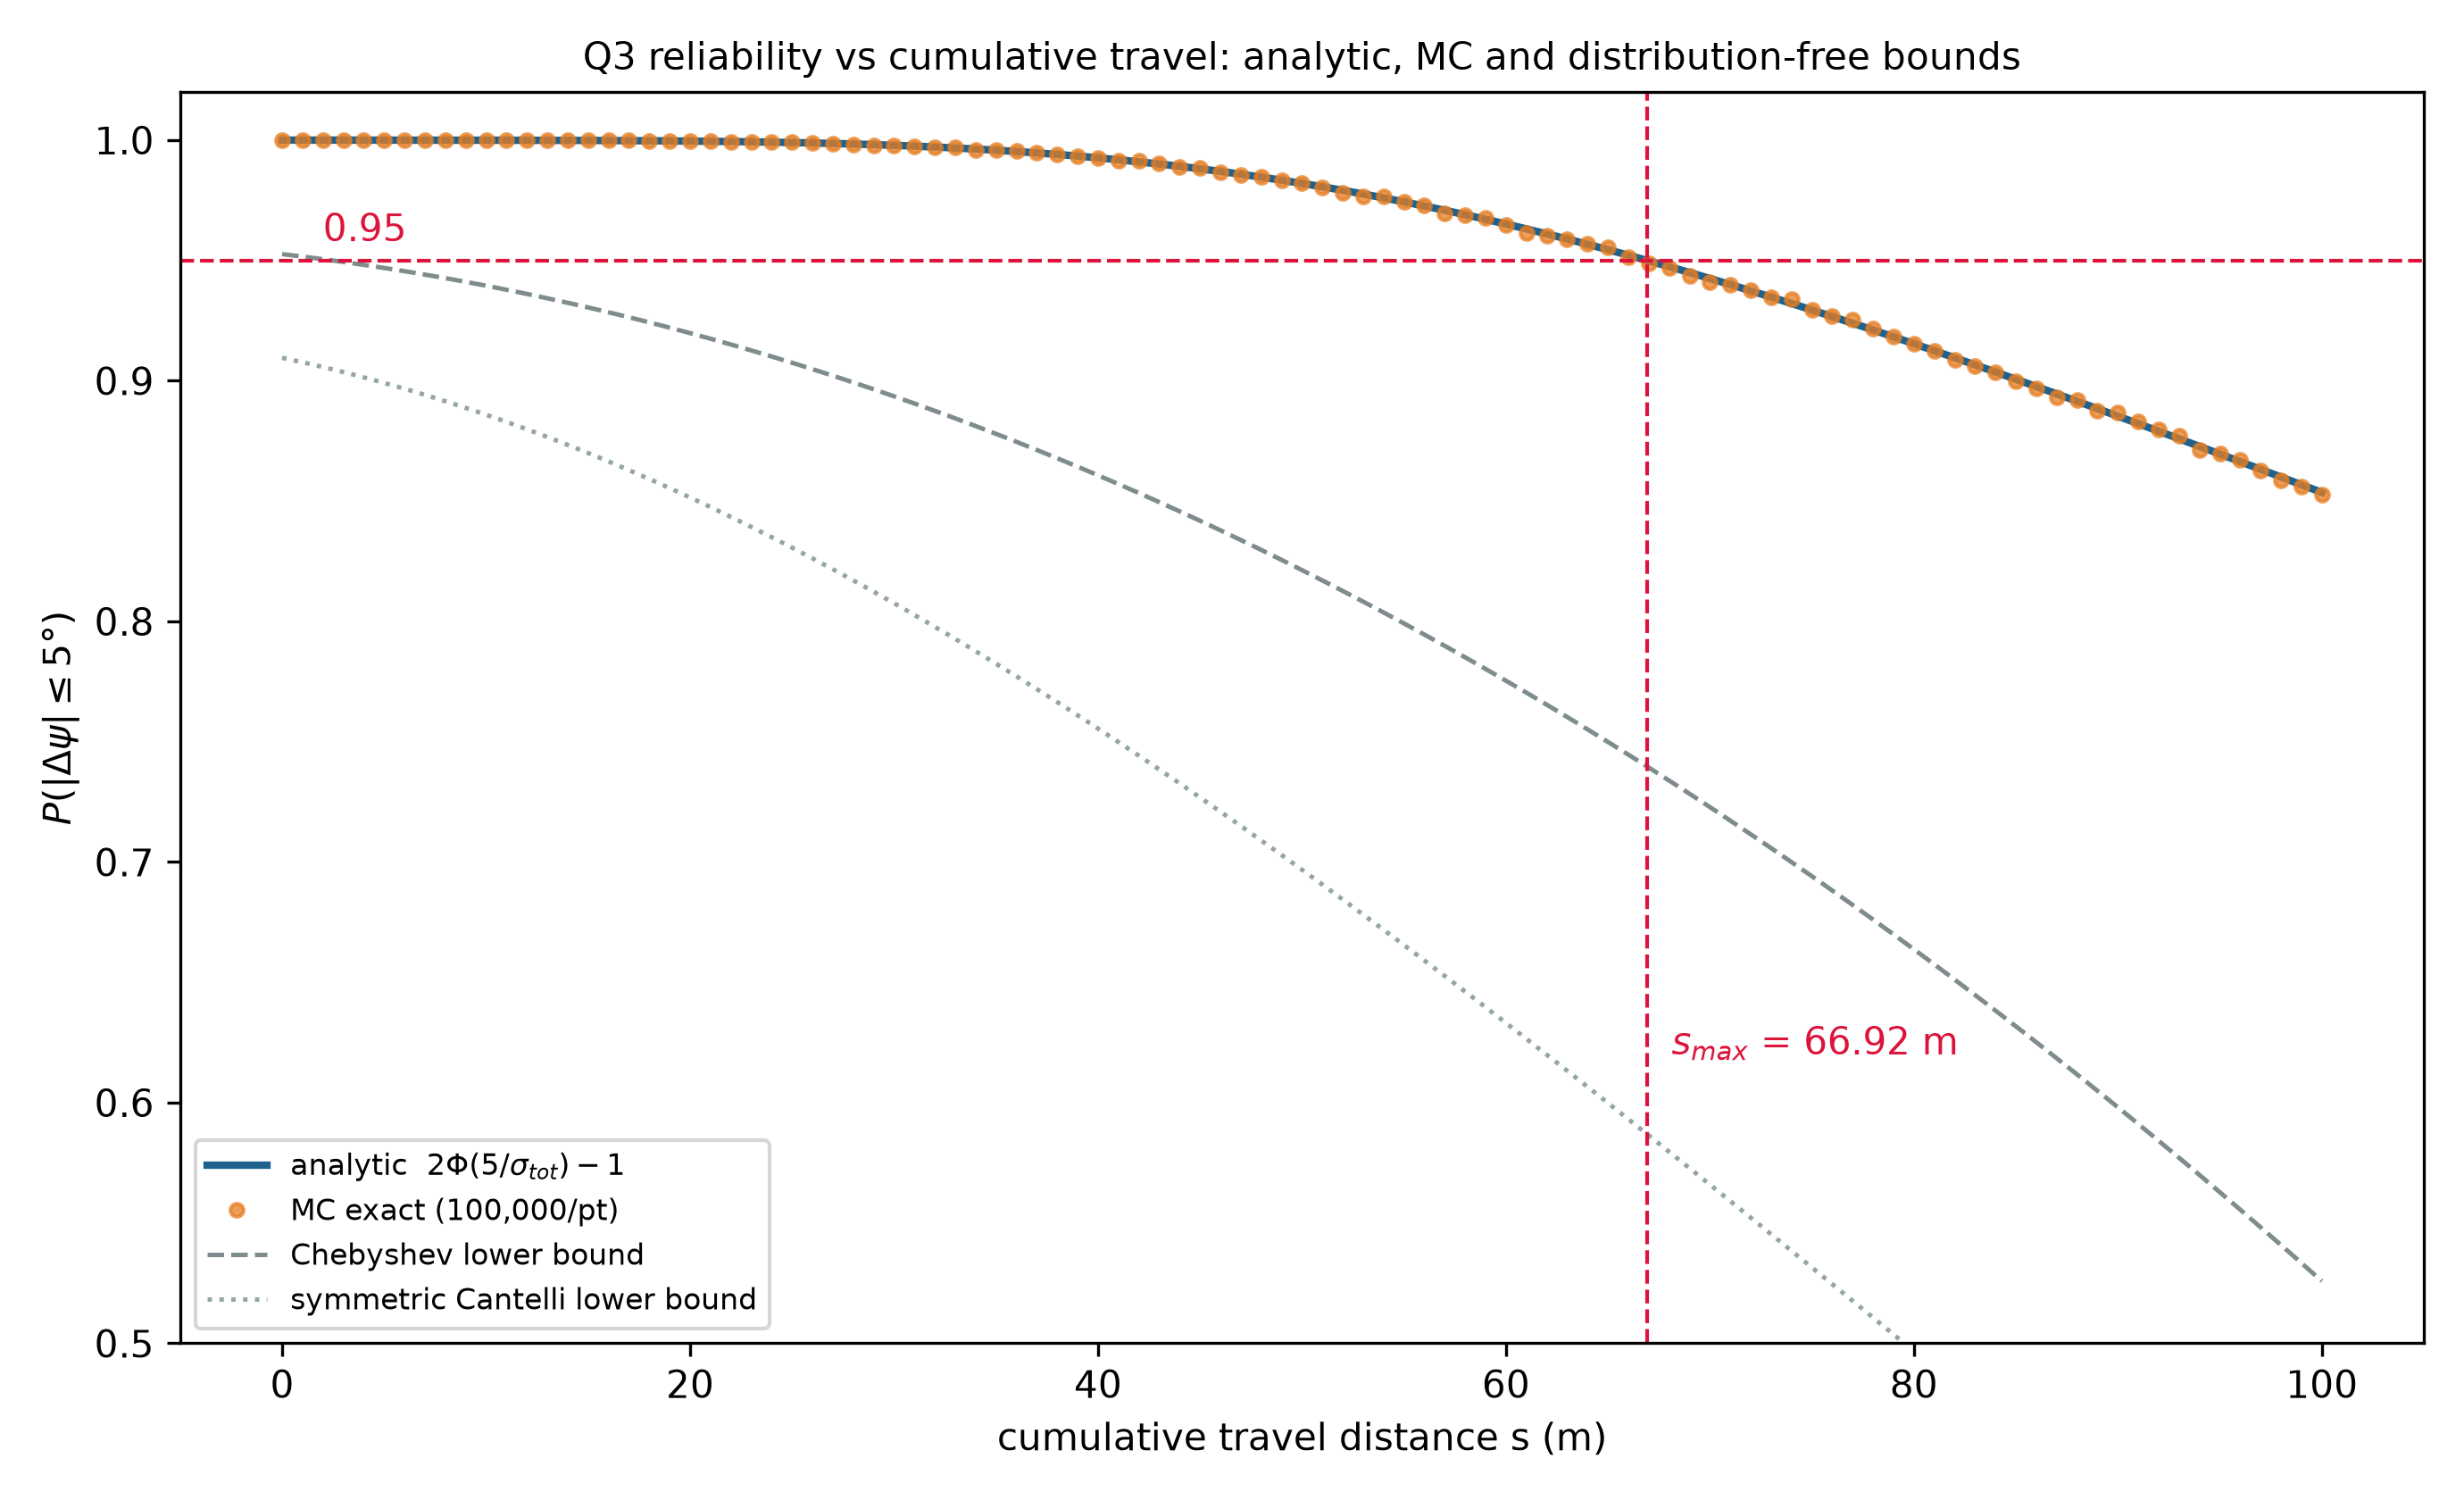
\includegraphics[width=0.39\textwidth]{fig_q3_p_s_curve.png}\hfill
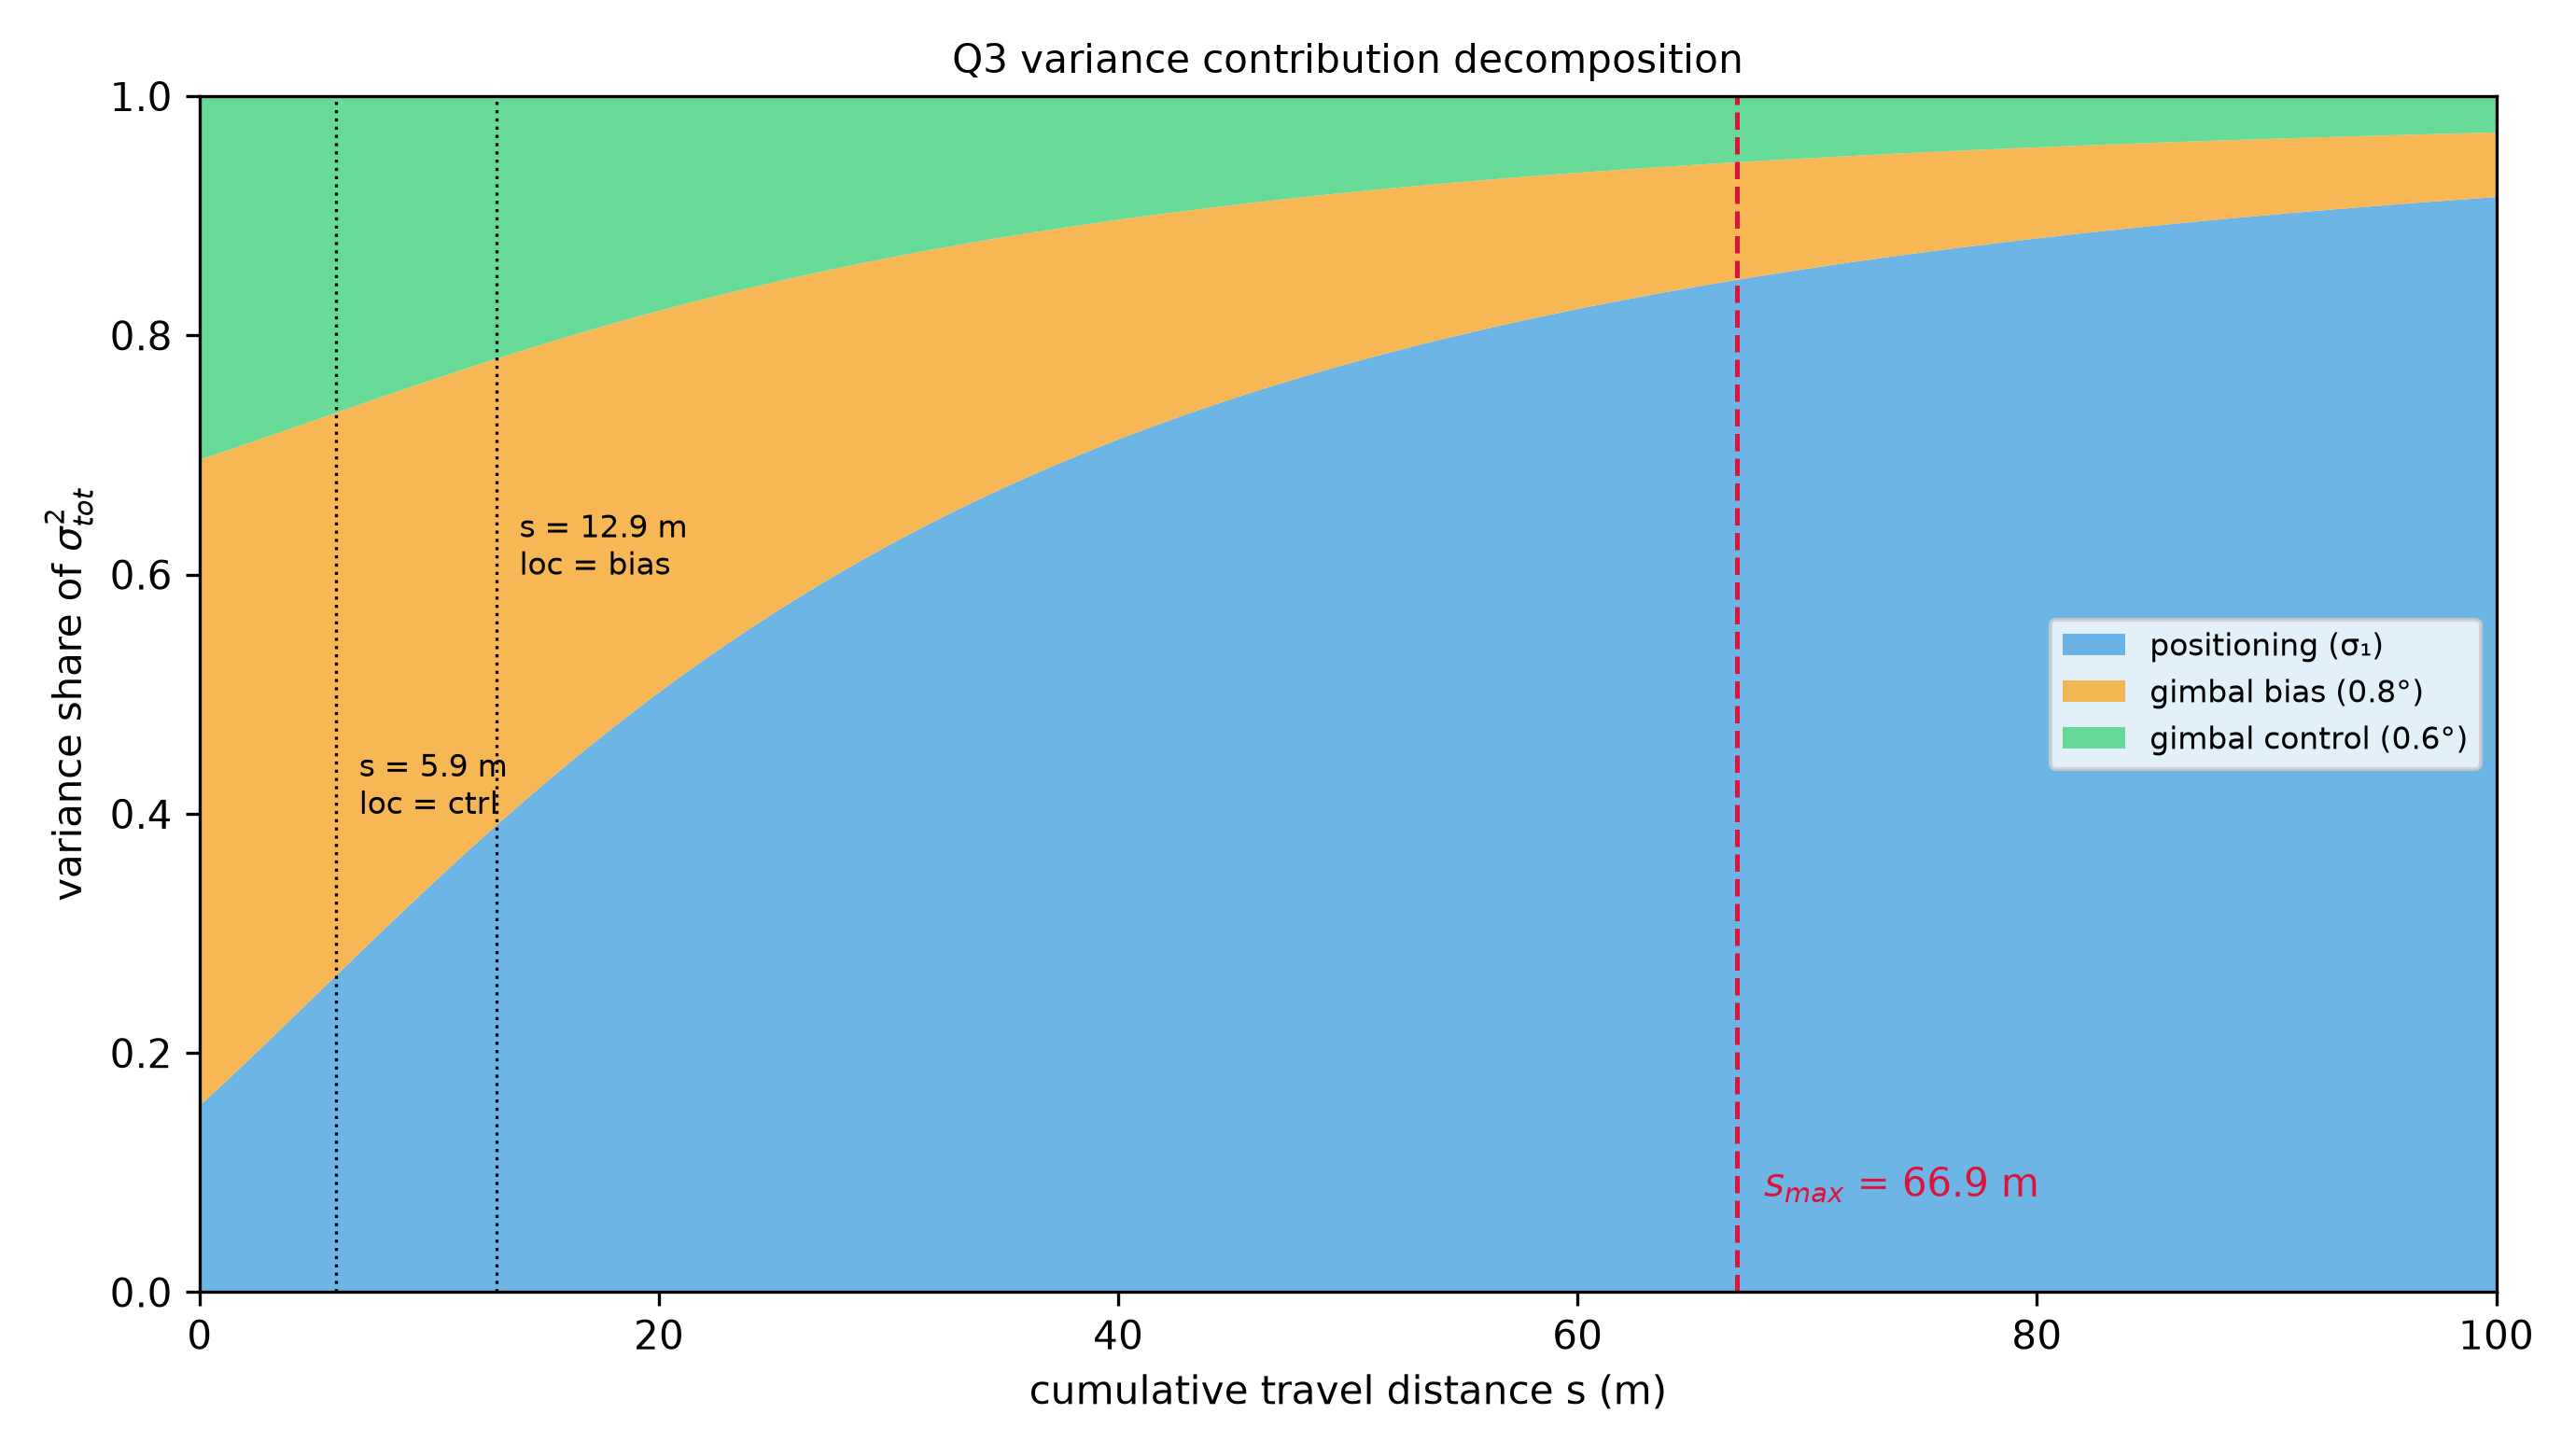
\includegraphics[width=0.39\textwidth]{fig_q3_contribution.png}
\caption{(a) Pointing reliability $P(|\Delta\psi|\le5^\circ)$ versus cumulative travel:
analytic chain (line) and exact-geometry Monte Carlo, $10^{5}$ samples per point, seed
2026 (dots); the dashed rule marks the $95\%$ requirement, crossing at
$s_{\max}=66.92\,\mathrm{m}$. (b) Variance-contribution decomposition along $s$: gimbal
zero bias dominates below $12.93\,\mathrm{m}$ (54.0\% at $s=0$), control error below
$5.94\,\mathrm{m}$; beyond $40\,\mathrm{m}$ the localization term owns $71.3\%$, rising
to $88.1\%$ at $80\,\mathrm{m}$.}
\label{fig:q3ps}
\end{figure}

Over $s\in[0,100]\,\mathrm{m}$, Fig.~\ref{fig:q3ps}a has maximum analytic--Monte Carlo
deviation $0.18$ percentage points; the interpolated Monte Carlo crossing is
$66.56\,\mathrm{m}$, $0.36\,\mathrm{m}$ below the analytic cap. At that cap,
Eq.~\eqref{eq:pexact} gives $P_{exact}=0.9497982$; a $5\times10^6$-sample exact-geometry
simulation gives $0.9498684$, Wilson 95\% CI \cite{wilson1927}
$[0.9496768$, $0.9500593]$. Solving $P_{exact}(s)=0.95$ gives $66.8373\,\mathrm{m}$,
where the same-size simulation gives $0.9500798$, Wilson interval $[0.9498886$,
$0.9502703]$.
Both intervals contain their quadrature targets.

The linearized cap exceeds the exact crossing by $0.0850\,\mathrm{m}$, hence is slightly
\emph{non-conservative}, although the reliability difference is only $0.0202$ percentage
points. We retain $66.9223\,\mathrm{m}$ as the analytic answer, report the full-geometry
bound as $66.8373\,\mathrm{m}$ ($66.84\,\mathrm{m}$), and deploy at $66.83\,\mathrm{m}$
without rounding upward. At $80\,\mathrm{m}$, baseline reliability is $91.5376\%$
(linearization) and $91.5068\%$ (full geometry): an 80-m approach is infeasible.

Chebyshev's distribution-free bound is only $2.45\,\mathrm{m}$; symmetric Cantelli is
infeasible because $\sigma_{tot}^2\le0.641$ is below the fixed gimbal variance $1.0$.
Figure~\ref{fig:q3ps}b gives crossovers at $5.94\,\mathrm{m}$ (control) and
$12.93\,\mathrm{m}$ (bias); localization owns over half the variance beyond
$19.91\,\mathrm{m}$.

\textbf{Deployment insight (feeding Q2/Q4).} The strict $66.83\,\mathrm{m}$ cap binds
before Q2(1)'s 90-m driving budget, so travel must stay below it or tasks must rotate.
All reported schedules comply; Q2(2)'s legs span $0$--$19.1\,\mathrm{m}$.
